% !TeX root = ../main.tex

\chapter{VAR Analysis}

We estimate the response for a GPR shock using a structural VAR model. Follow \citet{caldara} settings, using two lags and quarterly data, and slightly changed to make all varialbles stationary following \citet{brignone}. Specifically, we take log-difference transformation of real fixed private investment and real TAIEX, take first diferences of policy rate, while party support rate and VIX remain levels. The log of private hours per capita is season adjusted consider Chinese New Year. The party support is the support rate of pro-DPP parties, indicates the government's support rate among data range. 

The Results are almost opposite to traditional expectation to GPR shock. Investment, work hours, TAIEX returns and party support all response to increase, even VIX becomes lower in short-term. This might come from China+1 effect. GPR shocks such as US-China trade-war and Covid-19 both push companies to find substitution of China and Taiwan enjoys the benefits to become one of the substitution. The real cause needs further investigation, but it would be interesting to research on Trump's 2025 tariff, as the tariff push suppliers to find other substitutions other than Taiwan.

\begin{figure}[htbp]
  \centering
  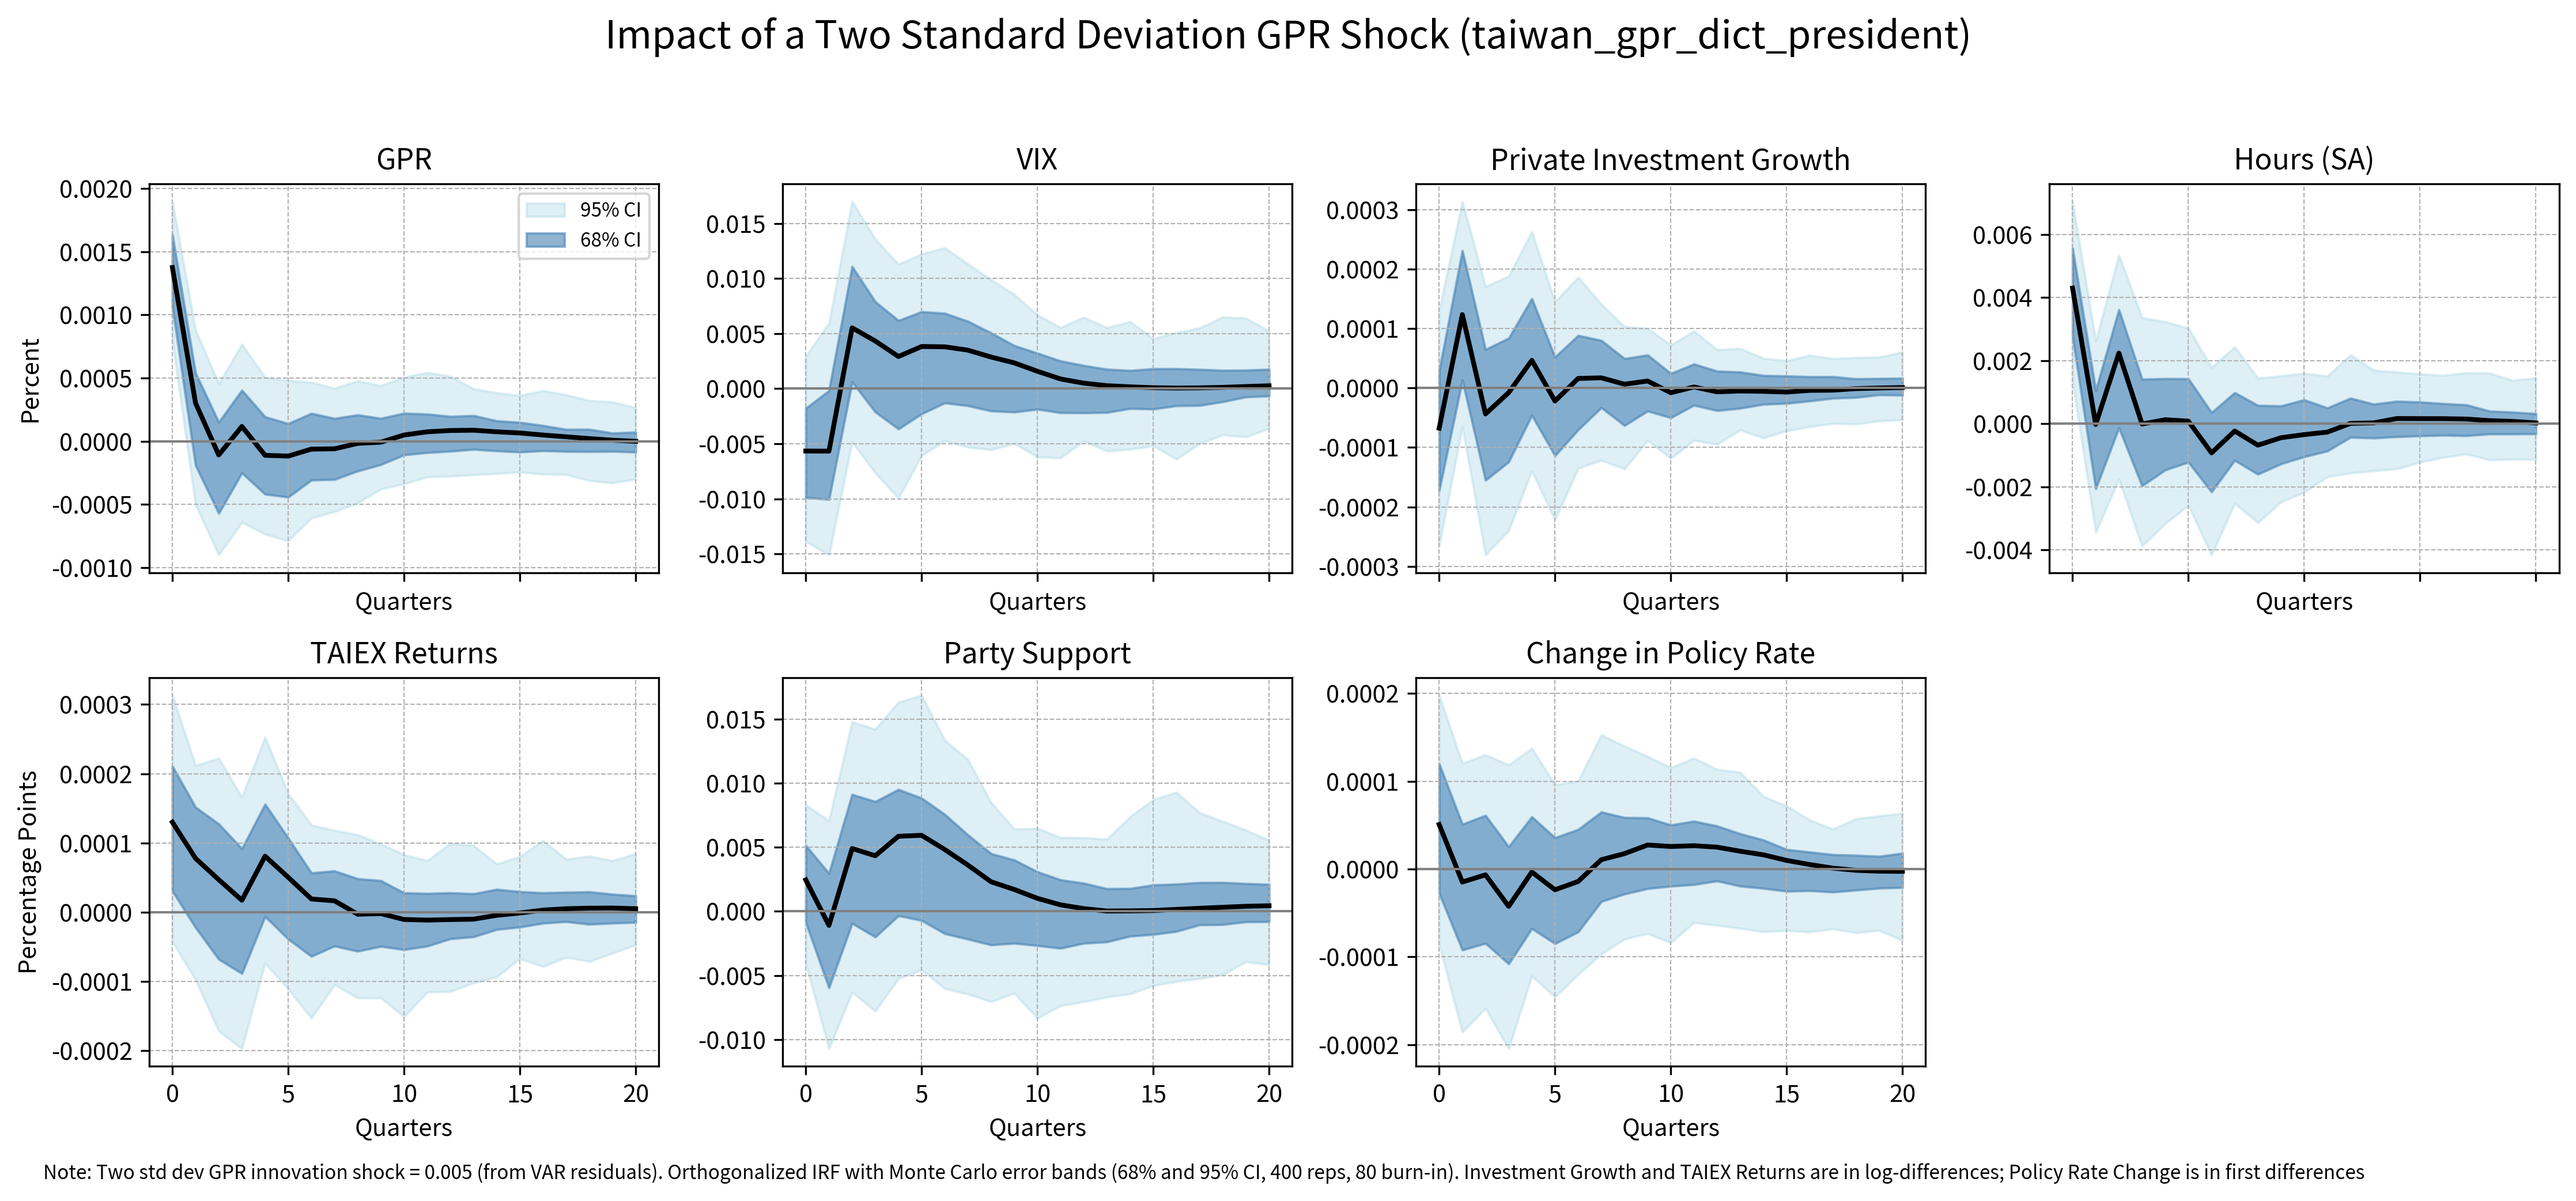
\includegraphics[width=\linewidth]{svar_irf_custom.png}
  \caption{The Impact of Increased Geopolitical Risk}
  \label{fig:my_example}
\end{figure}